\documentclass[../stegner_thesis.tex]{subfiles}

\begin{document}

\chapter{Methodology}%
\label{ch:methods}

\section{Threat Model}%
\label{sec:mthd_threat_model}

\par A vital part of addressing any cyber security threat is defining the
threat model.
Without a specific threat model, the problem space is difficult to define.
In our threat scenario, a malicious actor causes some software from a 3rd party
vendor to perform some malicious action.
We require a context-aware malware analysis model to detect such malicious
software before it is run on an autonomous drone.
A diagram of our threat model is shown in \figref{fig:threat_model}.

\begin{figure}[htb]
	\centering
	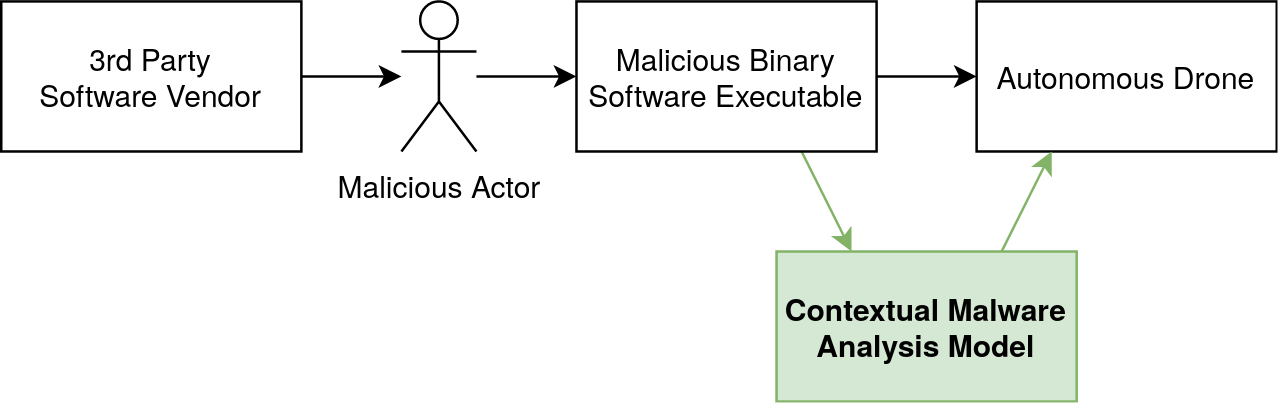
\includegraphics[width=0.75\textwidth]{img/threat_model.png}
	\caption[Threat model diagram]{Threat model diagram.}%
	\label{fig:threat_model}
\end{figure}

\section{Context Definition}%
\label{sec:mthd_context_def}

\par One of the biggest challenges in this work has been defining context.
In \secref{sec:bg_context}, existing literature regarding context in
software analysis is discussed.
However, these works do not define context in a way which aligns with the goals
of this work.
In order to properly address context, we want to address the following
questions:

\begin{enumerate}
	\item What is the physical context of the system (e.g., location and
		altitude)?
	\item How does the actual behavior compare to the expected behavior?
	\item Why is the software making certain decisions?
\end{enumerate}

\par The physical context is an important component of context, especially for
mobile systems, such as autonomous drones.
For instance, if a drone performs a specific action, it may be difficult to
tell if that action is benign or malicious without considering factors such
as its position, altitude, or external weather conditions to name a few.
Recall the autonomous drone example from \secref{sec:intro_motivation}; turning
the camera off in some areas may be beneficial for preserving sensitive data,
while turning the camera off in other areas can be malicious if the purpose is
to obstruct the gathering of intelligence.
The simple act of turning the camera off is not inherently malicious, but the
physical conditions which caused the camera to turn off can indicate whether
the act was malicious or benign.

\par Understanding the expected behavior of a program is foundational for
developing context because it defines what actions are expected.
For example, it makes sense for a text editor to read and write files on the
system because that is part of the expected behavior, and modifying files fits
the context.
It would probably be unexpected for a text editor to start recording from a
webcam because that behavior does not fit the context of a text editor.
In contrast, a program designed for video calls would be expected to access
the web cam because that fits the context of a video call software.
The act of accessing the webcam cannot be labeled as malicious or benign
without knowledge of what the program should be doing.

\par Perhaps the most fundamental question in determining the context of a
program is why it makes certain decisions.
This question is much broader and more difficult to address precisely than the
previous two.
When a human expert examines a piece of software to determine whether or not
it is malware, they are looking not only at what behaviors are present, but
looking at what conditions will cause such behaviors to occur.
The human expert can then rely on domain knowledge and previous experience to
determine if the actions are malicious or benign.

\section{Cross Validation}%
\label{sec:mthd_cross_valid}

\par Due to the random nature of fitting LDA models, we observed high
variation in the accuracy of classifiers which use the LDA features as their
primary features.
To tune the parameters of the models, it is important to know whether
differences in classification accuracy are due to randomness in the fitting
process or if the parameters are actually better.
To get a better evaluation of the classifiers, we applied k-fold cross
validation~\cite{hastieElementsStatistical}.
The k-fold cross validation process is described by \algref{alg:k_fold}.

\begin{algorithm}[H]
	\caption{k-Fold Cross Validation}%
	\label{alg:k_fold}
	\KwData{Dataset $D$}
	Randomly shuffle $D$\;
	Split $D$ evenly into $fold_{0}$, $fold_{1}$, \ldots $fold_{k-1}$\;
	\For{$i \gets{} 0$ \KwTo{} $k-1$}{%
		Initialize a new model\;
		Fit model on $D \setminus fold_i$\;
		Evaluate model accuracy on $fold_i$\;
	}
	Compute mean and standard deviation accuracy\;
\end{algorithm}

\par An alternative validation strategy is holdout validation.
In this strategy, only a single model is fitted with set testing and training
partitions, which takes less time than cycling through all of the folds.
However, k-fold cross validation is advantageous over holdout validation in our
case because multiple models are trained, allowing us to observe the mean
classification accuracy and standard deviation.
By testing the models on multiple distinct testing sets, we are able to make
stronger claims about the performance of our models.

\section{Datasets}%
\label{sec:mthd_datasets}

\subsection{Das Malwerk Dataset}%
\label{subsec:mthd_das_malwerk}

\par For evaluating our first context-aware model, we wanted a simple dataset
for preliminary testing.
We also had an initial requirement to use live files to collect dynamic
features.
This requirement was later dropped from the model, but the dataset was chosen
under constraint of needing live files.
To meet these requirements, we collected malicious files from Das
Malwerk~\cite{svenssonMalwerk} and benign files from a default installation of
Windows 7.
This dataset was chosen because of its small size and the fact that it
contains live executable files, meaning it met our requirements.
This dataset contains 576 malicious files and 646 benign files.

\par To get the dataset into a usable state, there were several preprocessing
steps.
First, the static assembly commands were obtained using
\texttt{objdump}~\cite{ObjdumpLinux}.
Given an input file \texttt{IN\_FILE} and a target output file
\texttt{OUT\_FILE}, \texttt{objdump} can generate the disassembly using the
\texttt{-d} flag as follows (on Linux systems):

\lstinputlisting[language=Bash]{code_samples/objdump.sh}

\par Next, the static assembly commands must be filtered down to documents
consisting of sequences of opcodes.
To achieve this, several command line utilities are piped together as a series
of string stream filters.
The first is \texttt{cat}~\cite{CatLinux}, which concatenates files and dumps
the output to standard output of the terminal.
Next, \texttt{sed}~\cite{SedStream} filters the incoming stream based on
regular expressions and puts the filtered stream in standard output.
Lastly, the \texttt{cut}~\cite{CutLinux} utility is used to isolate the column
of the remaining output which contains the opcodes.
The process of taking an input file \texttt{IN\_FILE} (the output from
\texttt{objdump}), filtering out the opcode sequence, and outputting it to the
output file \texttt{OUT\_FILE} is as follows (again, on Linux systems):

\lstinputlisting[language=Bash]{code_samples/filter_das_malwerk.sh}

\par The resulting sequences of opcodes are used as documents for the models
discussed in this study.

\subsection{Microsoft BIG 2015 Dataset}%
\label{subsec:mthd_msoft_big}

\par After preliminary experimentation, we found several drawbacks with the
Das Malwerk dataset we wanted to fix for further testing.
The biggest drawback is that the Das Malwerk dataset consists of only two
classes, and each class contained a very broad mix of types of software.
The benign class had all of the executable files found on a default Windows 7
installation, which includes web browsers, text editors, media players, and
many others.
Furthermore, the malicious class includes a mixture of unsorted malware
programs, and sorting them into more specific groups would have been a manual
process prone to error.
With such drastically different functionality, it does not make sense to assign
a single acceptable context to each class.
The scenario was just too simple.

\par To improve our methodology, we needed a better dataset.
The new dataset must have multiple classes which are separated by specific
program type, and not just into malicious and benign classes.
We no longer had the constraint of needing live files because the dynamic
analysis components had been set aside, which gave us more dataset options.
To meet these requirements, the second dataset we used was the Microsoft
Malware Classification Challenge (BIG 2015) malware
dataset~\cite{ronenMicrosoftMalware2018}.
This dataset has become a benchmark for malware detection algorithms, and it
has been widely studied.
The details of the class distribution of the BIG 2015 dataset are shown in
\tabref{tab:big_2015_details}.

\begin{table}[htb]
	\centering
	\caption[BIG 2015 dataset details]{%
		Details of the BIG 2015 dataset class distributions.
	}%
	\label{tab:big_2015_details}
	\begin{tabular}{l c c}
		\toprule
		Class Name & Class ID & Number of Samples \\
		\midrule
		\midrule
		Ramnit~\cite{Win32Ramnit} & 1 & 1541 \\
		Lollipop~\cite{AdwareWin32} & 2 & 2478 \\
		Kelihos\_ver3~\cite{Win32Kelihos} & 3 & 2942 \\
		Vundo~\cite{Win32Vundo} & 4 & 475 \\
		Simda~\cite{Win32Simda} & 5 & 42 \\
		Tracur~\cite{Win32Tracur} & 6 & 751 \\
		Kelihos\_ver1~\cite{Win32Kelihos} & 7 & 398 \\
		Obfuscator.ACY~\cite{VirToolWin32} & 8 & 1228 \\
		Gatak~\cite{Win32Gatak} & 9 & 1013 \\
		\bottomrule
	\end{tabular}
\end{table}

\par One of the interesting challenges about this dataset is that the number of
samples varies by orders of magnitude between some classes.
We do not explicitly address this issue and leave it to future work, though
several existing studies have addressed the issue~\cite{%
	messay-kebedeCombinationTraditional2018,
	zhangUsingMultifeatures2016,
	yueImbalancedMalware2017,
}.

\par Preprocessing for the BIG 2015 dataset was much simpler than for the Das
Malwerk dataset because BIG 2015 was distributed in disassembly form.
Therefore, it only required filtering it down to a sequence of opcodes.
The opcodes were filtered out using regular expressions similarly to the Das
Malwerk dataset.

\section{Context-Free Model}%
\label{sec:mthd_context_free}

\par Before developing the context-aware models, we demonstrated that LDA
modeling is able to extract useful features from the dataset.
To do this, we tested a context-free malware classification model using LDA
features in a k-NN classifier.
The context-free model was also used to explore parameters of the LDA and k-NN
models, namely the number of topics in LDA and $k$ in k-NN\@.
Assuming we have each dataset such that each document is a sequence of opcodes
(done via preprocessing, described in \secref{sec:mthd_datasets}), the process
for creating the context-free model is as follows:

\begin{enumerate}
	\item Transform all documents into BoW documents.
	\item Fit LDA model on the training partition.
	\item Transform all BoW documents into topic distributions.
	\item Fit k-NN classifier on the topic distributions of the training
		partition.
	\item Evaluate k-NN classifier on the topic distributions of the test
		partition.
\end{enumerate}

\par To thoroughly evaluate this model, we use 5-fold cross validation as
described in \secref{sec:mthd_cross_valid}.
We limited the number of folds to five for model training time.
In the LDA models, we explored the effect of the number of topics, testing
values from 5 to 95 at multiples of 5.
For k-NN, we tested values for $k$ taking the odd numbers from 1 to 49.

\par To help understand the features generated by LDA, a 10 topic LDA model
was fit on the BIG 2015 dataset, and the learned topics are visualized as word
clouds in \figref{fig:wordcloud}.
Each topic is a probability distribution over the vocabulary of the corpus,
and the probability of each word is shown by the size of the word in the word
cloud.
The larger words should be interpreted as more significant to the topic, while
the smaller words are less significant.
Note how some topics, such as \figref{fig:wordcloud_topic_0}, seem to have only
a few words.
These topics still span the entire vocabulary, but the probability distribution
is heavily skewed toward a few of the words, and the rest of the words are so
insignificant to the topic that they are not large enough to be visible in the
word cloud.

\begin{figure}[htb]
	\centering
	\begin{subfigure}[c]{0.18\textwidth}
		\centering
		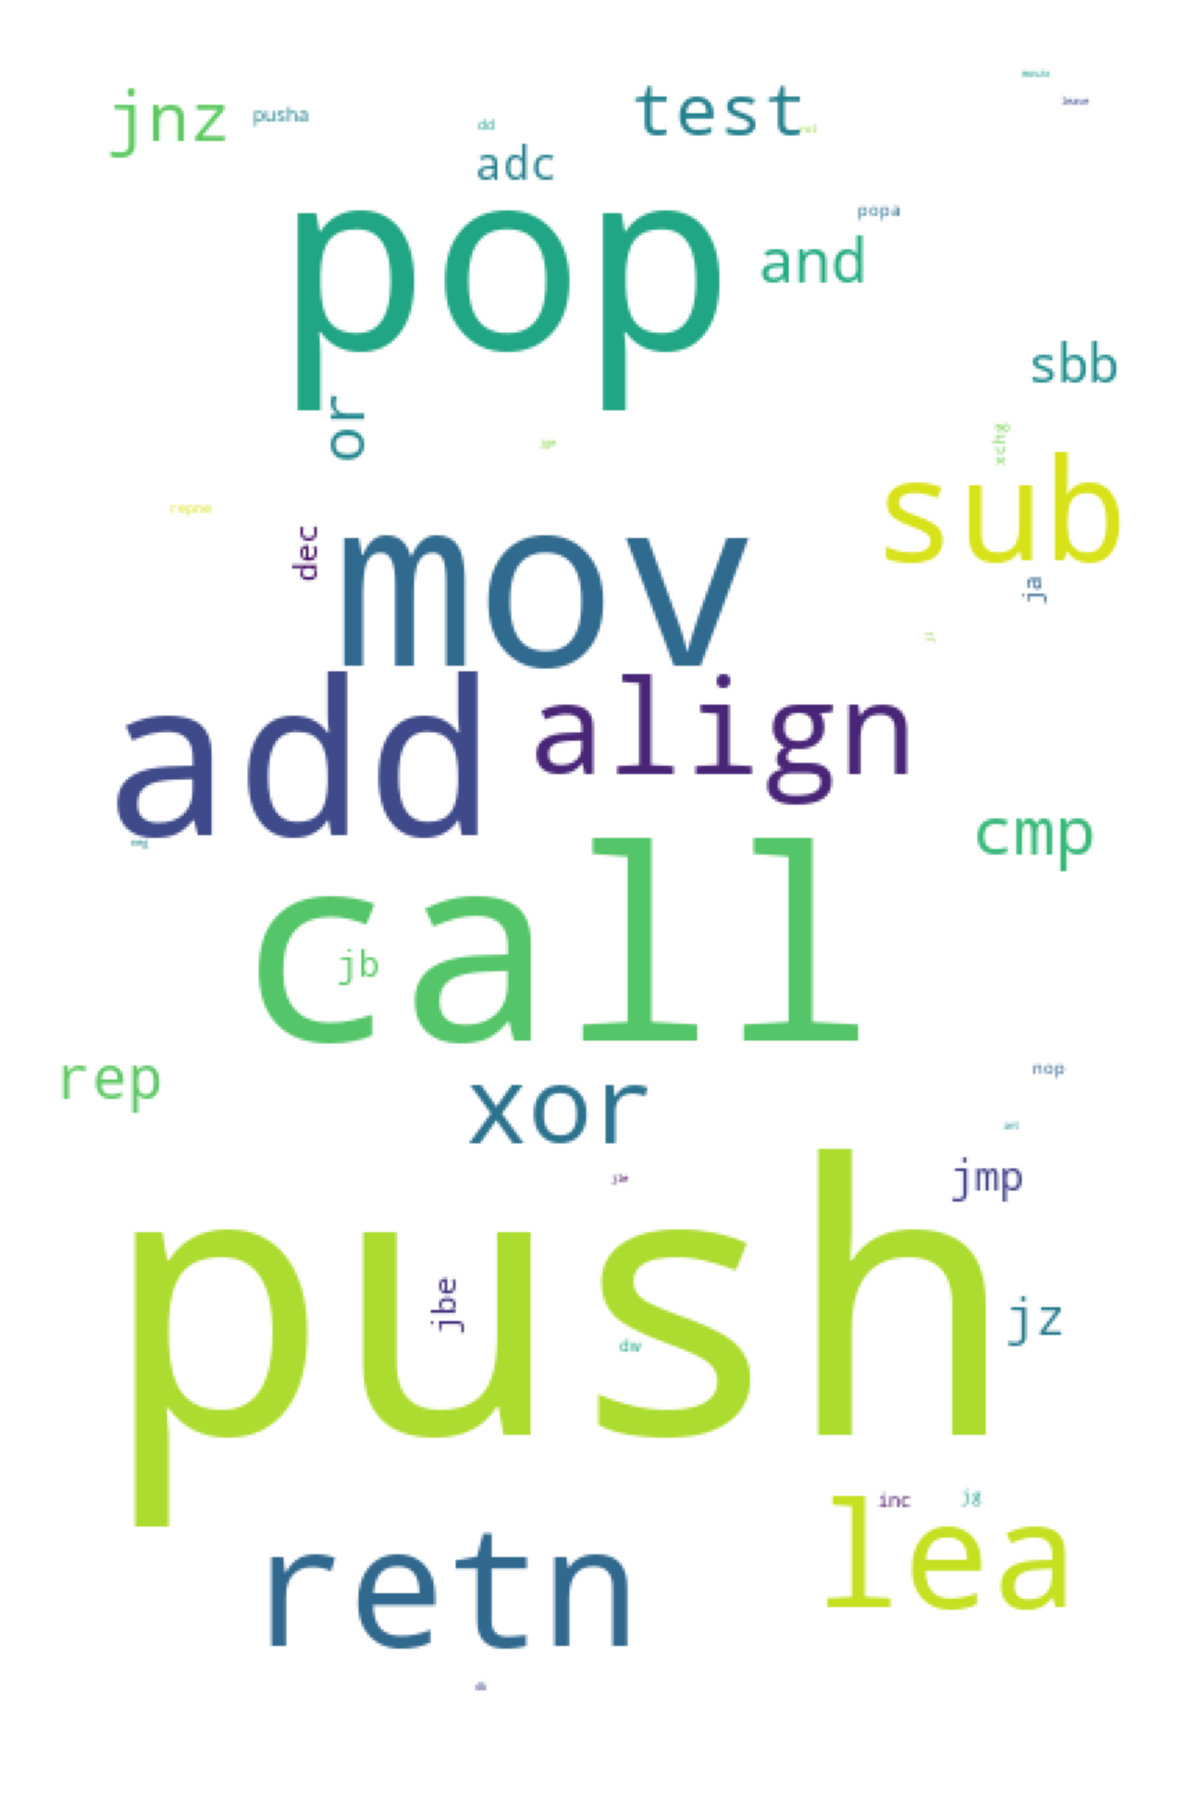
\includegraphics[width=0.95\textwidth]{%
			img/msoft_big/wordcloud/topic_00_wordcloud.png%
		}
		\caption{Topic 0.}%
		\label{fig:wordcloud_topic_0}
	\end{subfigure}
	\hfill
	\begin{subfigure}[c]{0.18\textwidth}
		\centering
		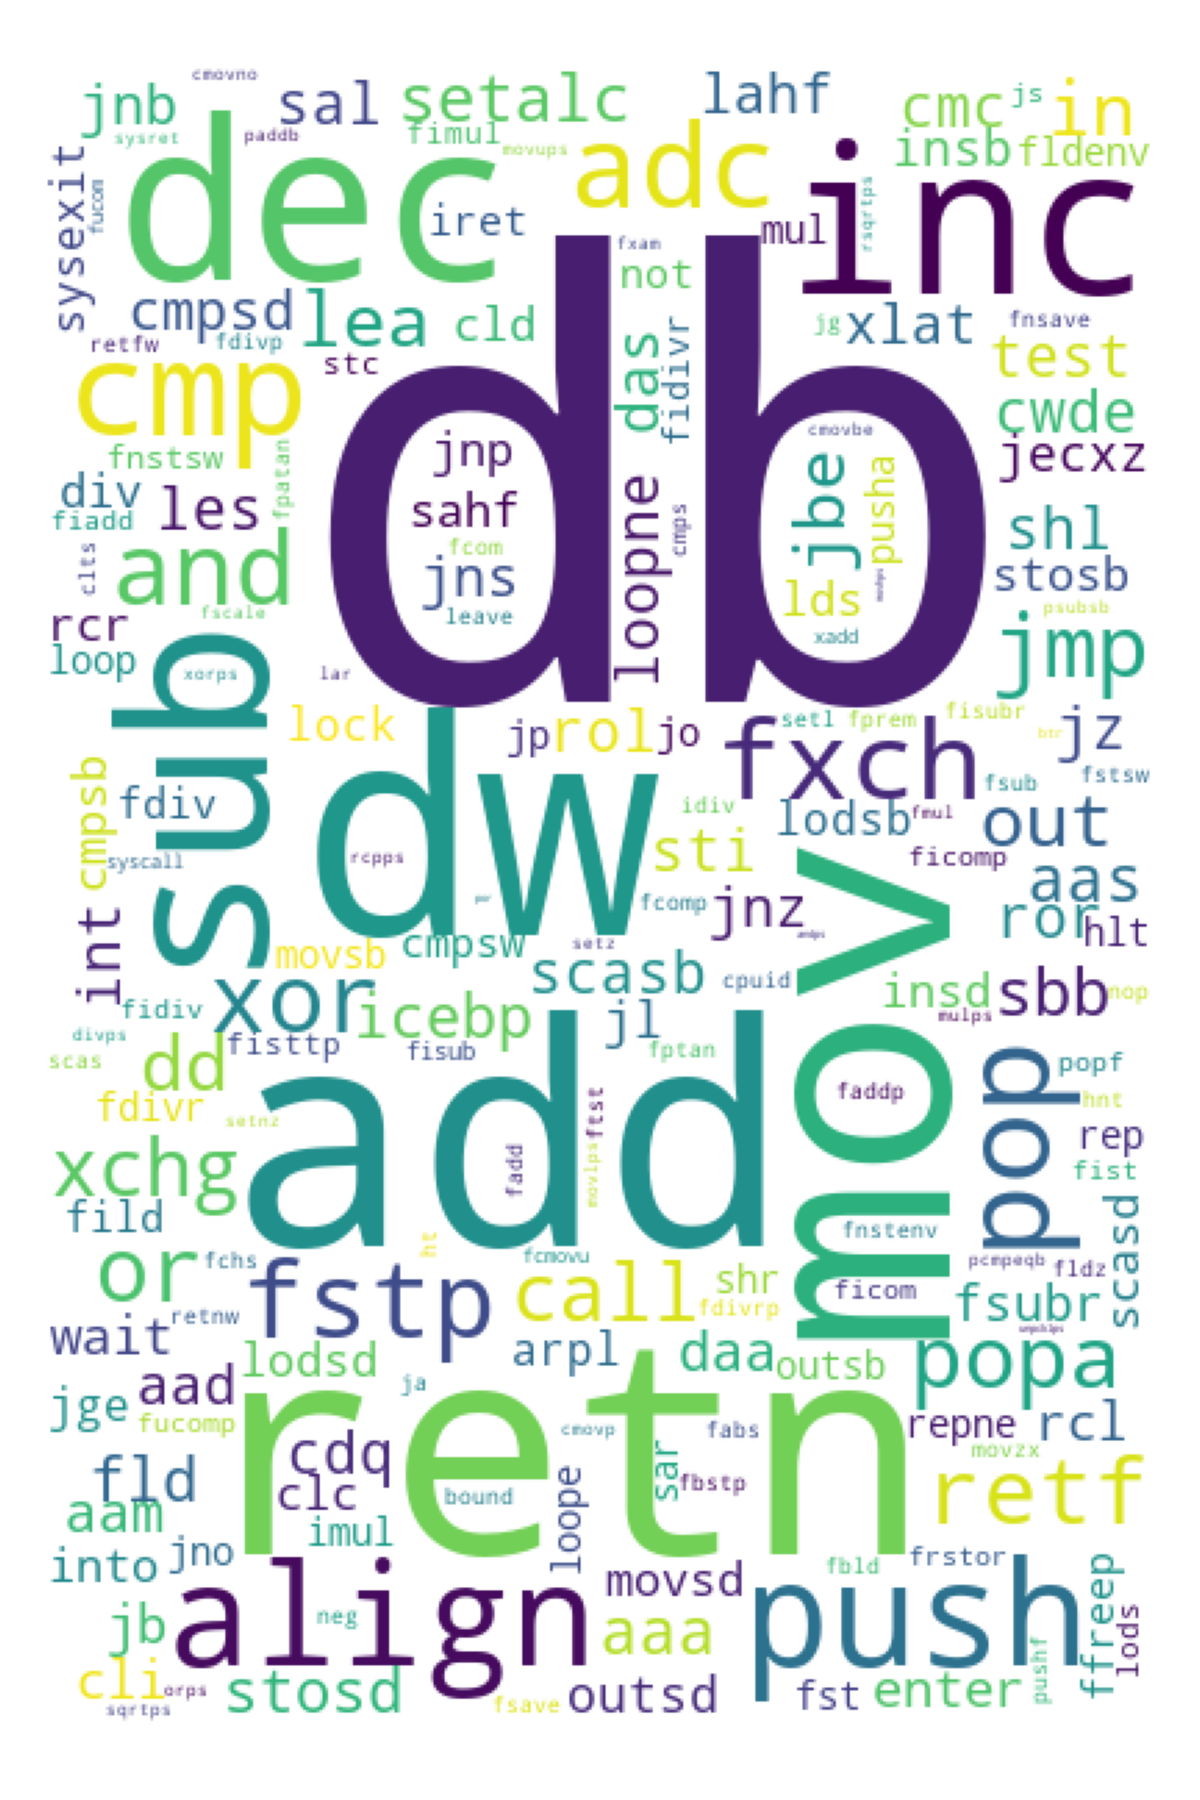
\includegraphics[width=0.95\textwidth]{%
			img/msoft_big/wordcloud/topic_01_wordcloud.png%
		}
		\caption{Topic 1.}%
		\label{fig:wordcloud_topic_1}
	\end{subfigure}
	\hfill
	\begin{subfigure}[c]{0.18\textwidth}
		\centering
		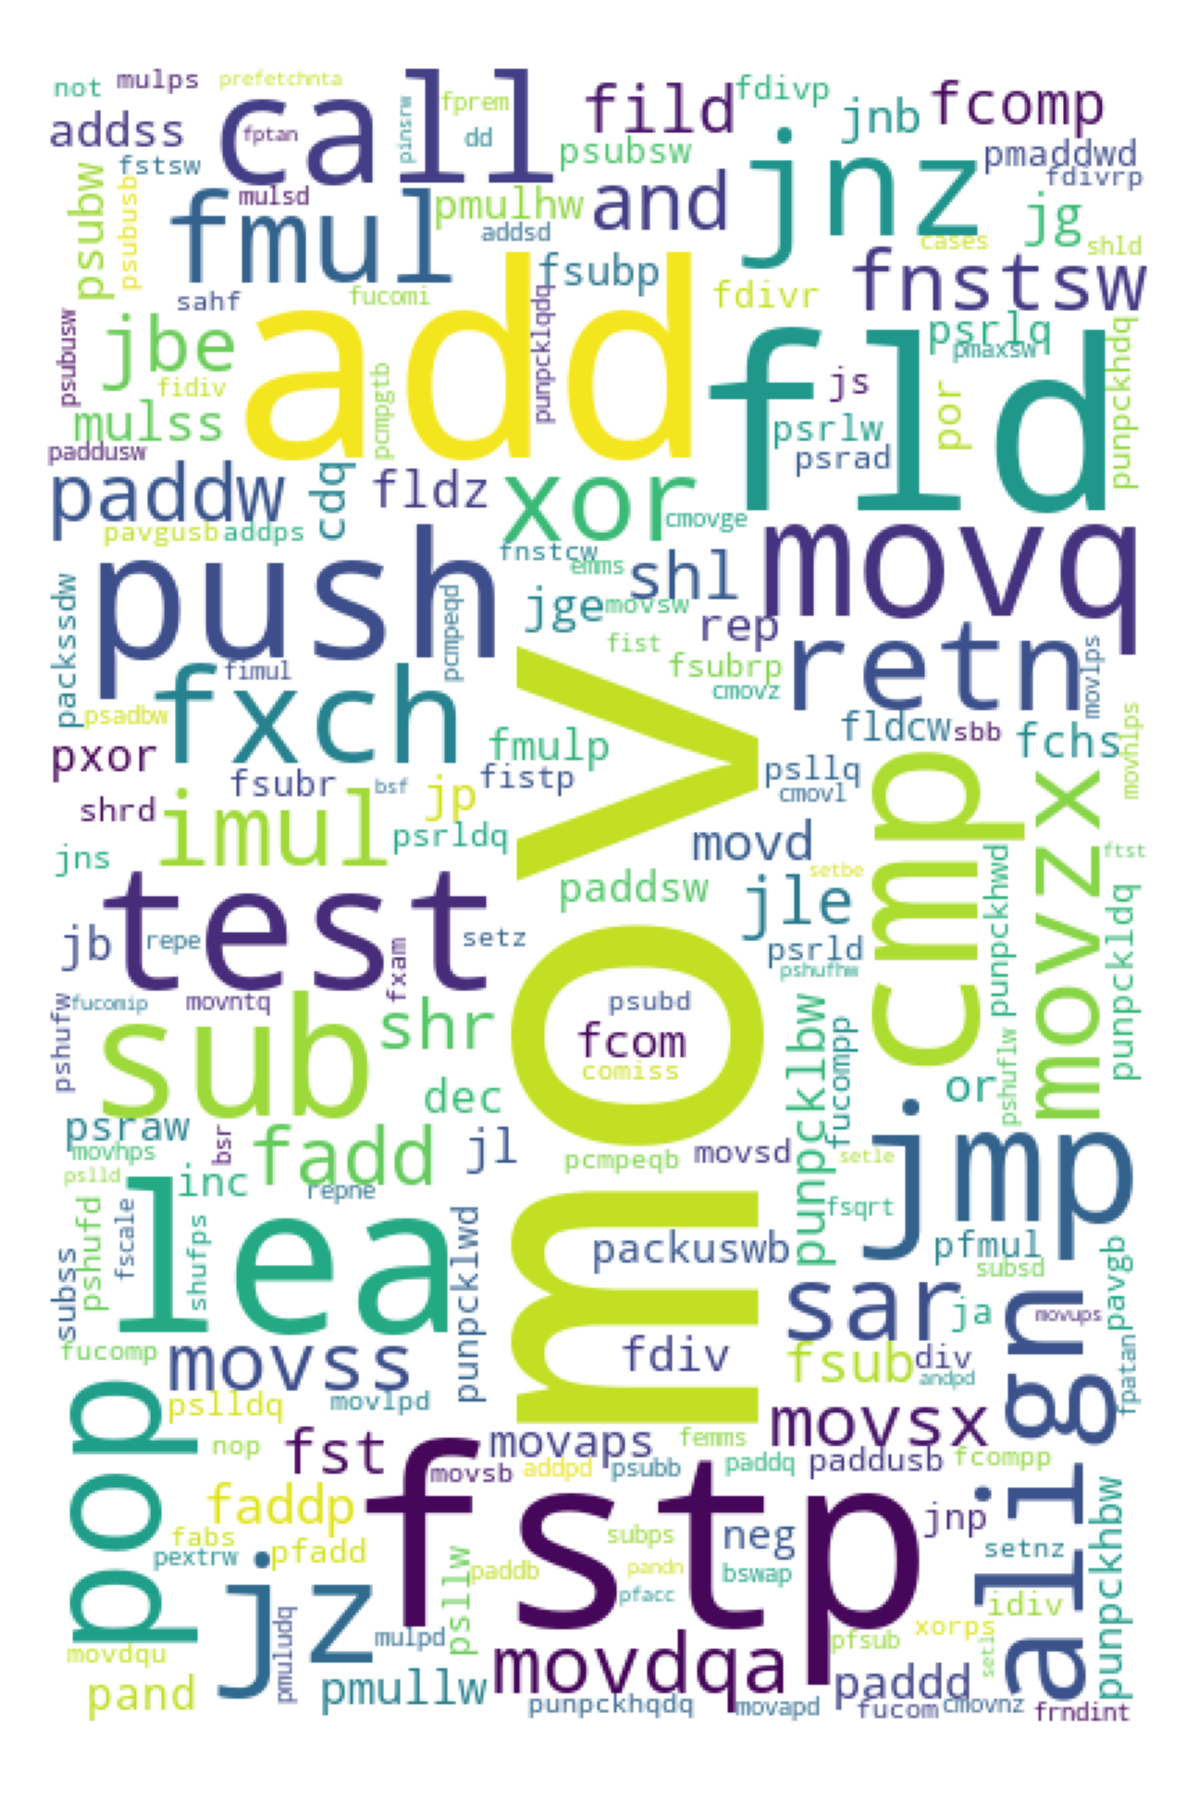
\includegraphics[width=0.95\textwidth]{%
			img/msoft_big/wordcloud/topic_02_wordcloud.png%
		}
		\caption{Topic 2.}%
		\label{fig:wordcloud_topic_2}
	\end{subfigure}
	\hfill
	\begin{subfigure}[c]{0.18\textwidth}
		\centering
		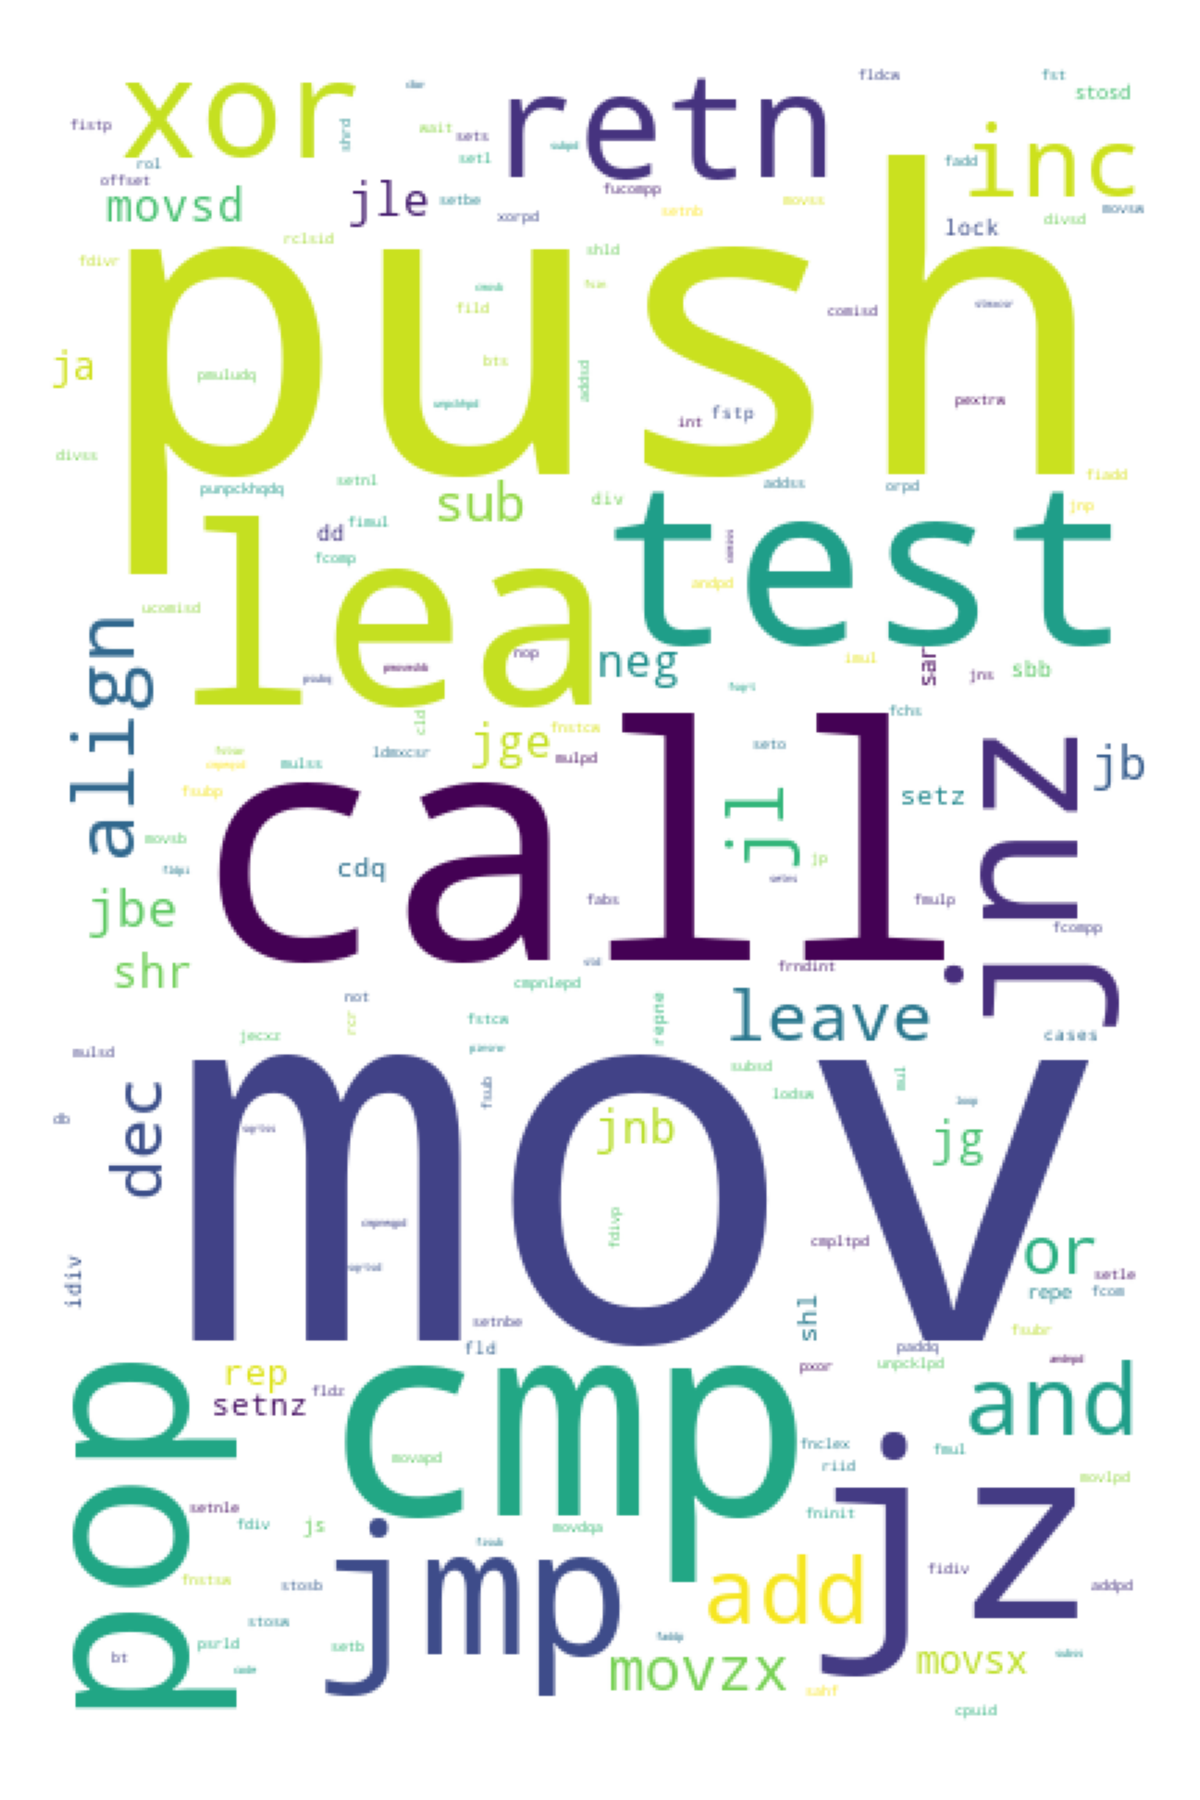
\includegraphics[width=0.95\textwidth]{%
			img/msoft_big/wordcloud/topic_03_wordcloud.png%
		}
		\caption{Topic 3.}%
		\label{fig:wordcloud_topic_3}
	\end{subfigure}
	\hfill
	\begin{subfigure}[c]{0.18\textwidth}
		\centering
		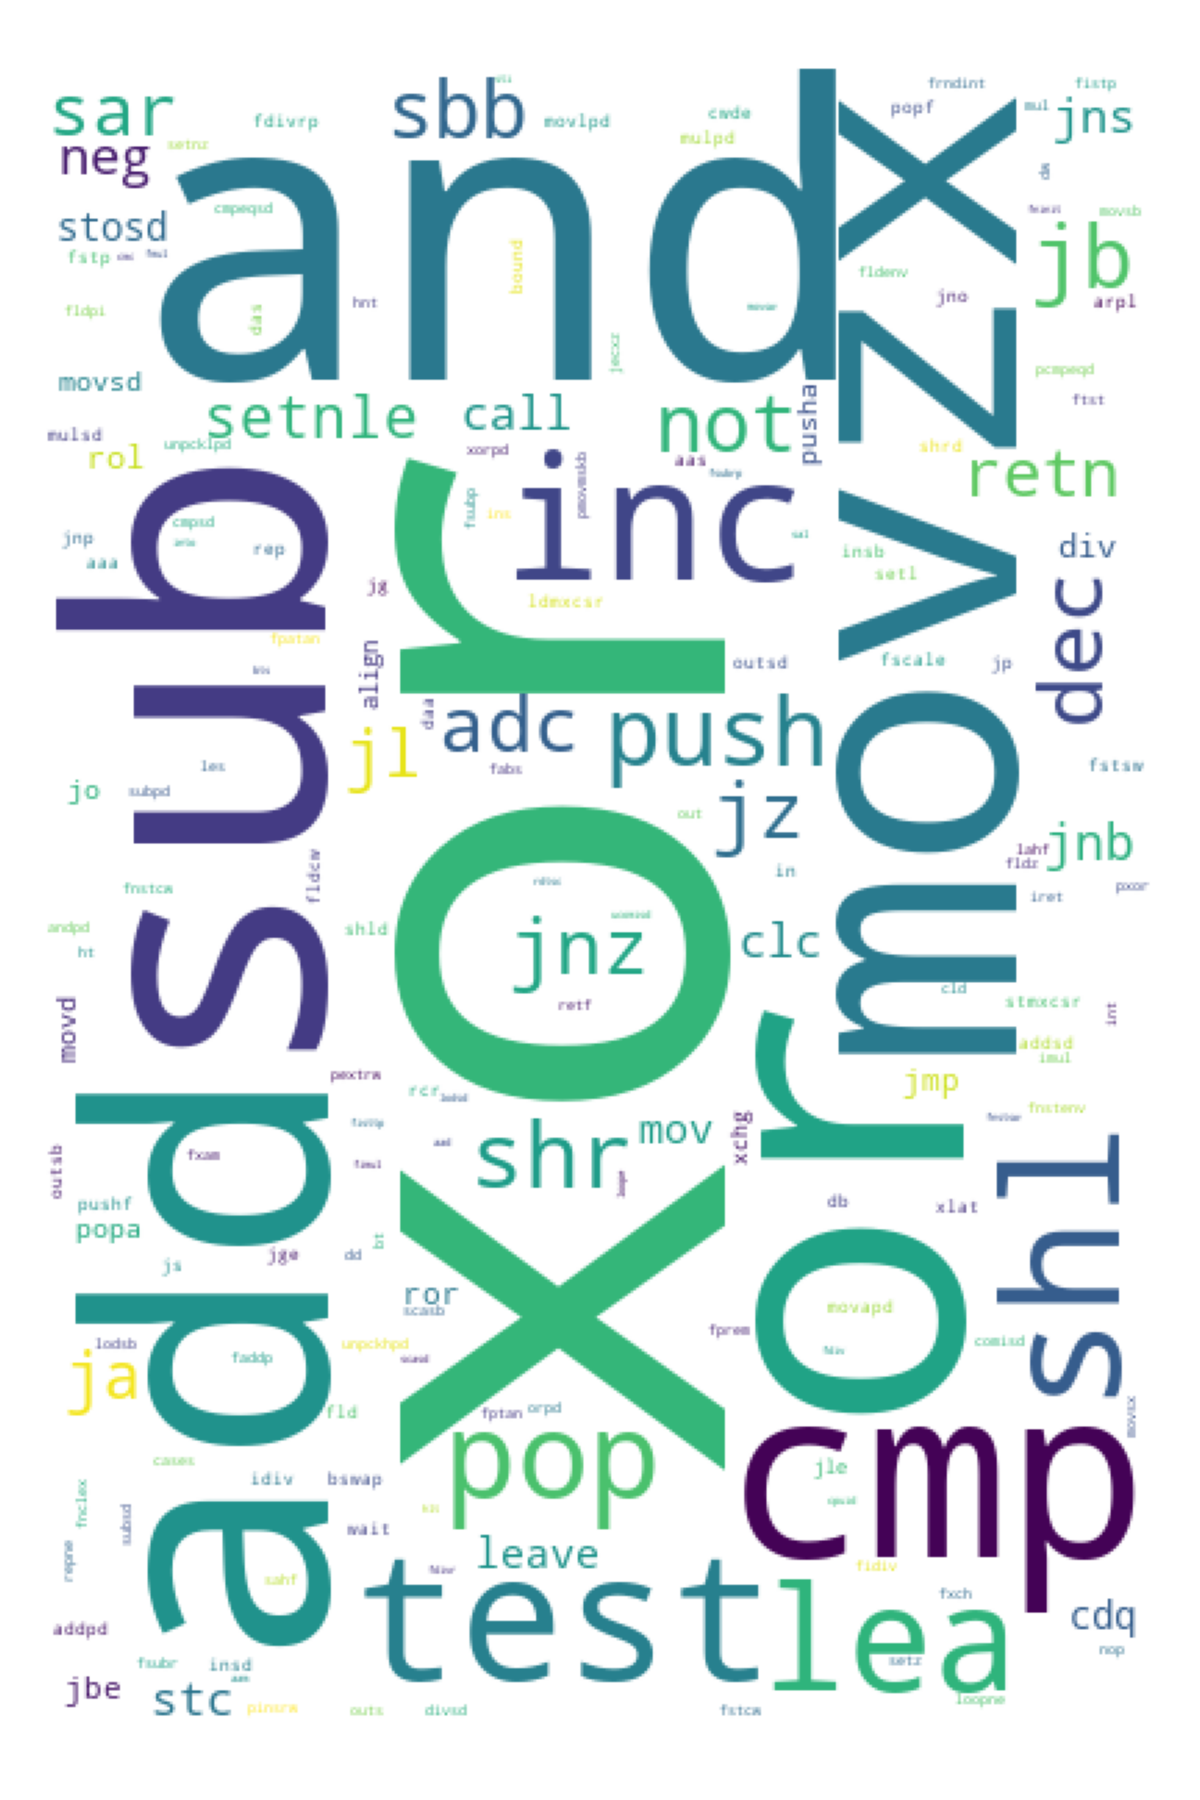
\includegraphics[width=0.95\textwidth]{%
			img/msoft_big/wordcloud/topic_04_wordcloud.png%
		}
		\caption{Topic 4.}%
		\label{fig:wordcloud_topic_4}
	\end{subfigure} \\
	\begin{subfigure}[c]{0.18\textwidth}
		\centering
		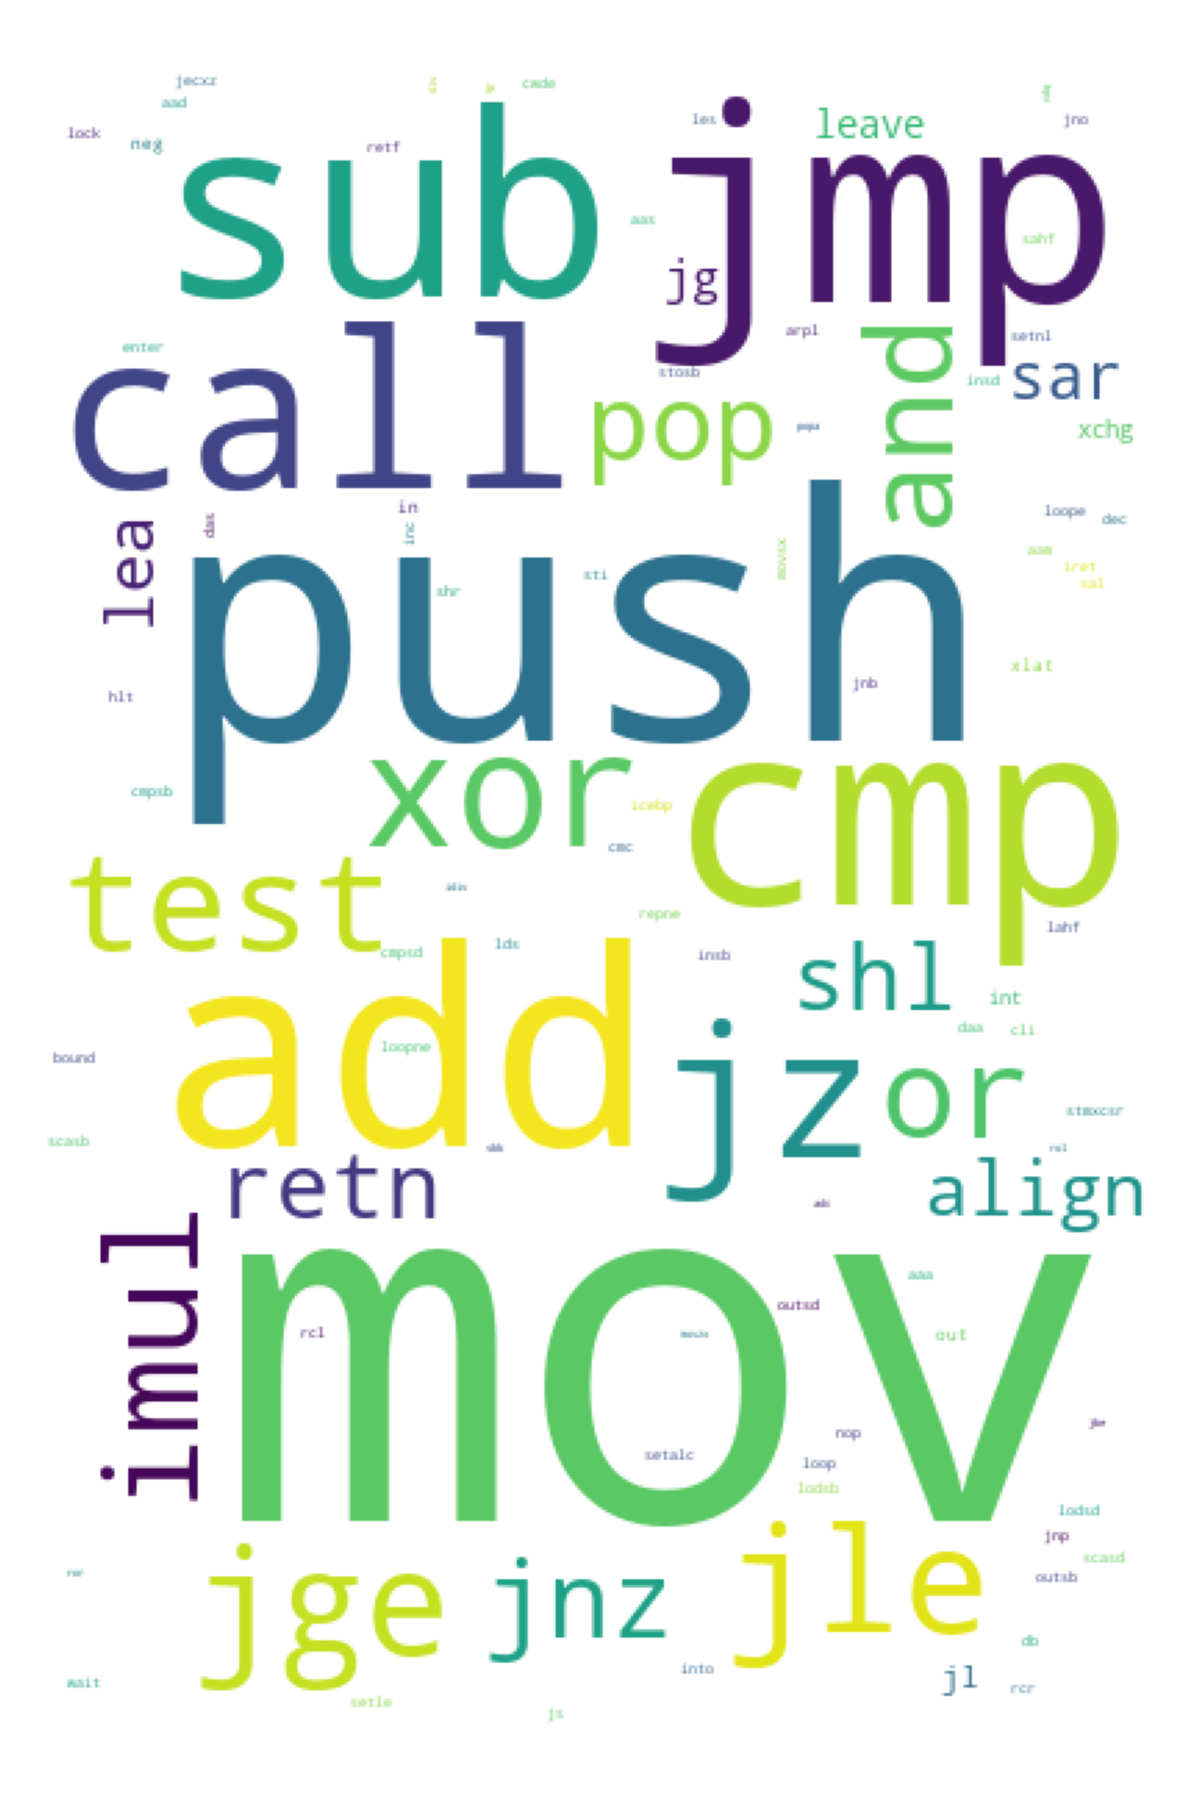
\includegraphics[width=0.95\textwidth]{%
			img/msoft_big/wordcloud/topic_05_wordcloud.png%
		}
		\caption{Topic 5.}%
		\label{fig:wordcloud_topic_5}
	\end{subfigure}
	\hfill
	\begin{subfigure}[c]{0.18\textwidth}
		\centering
		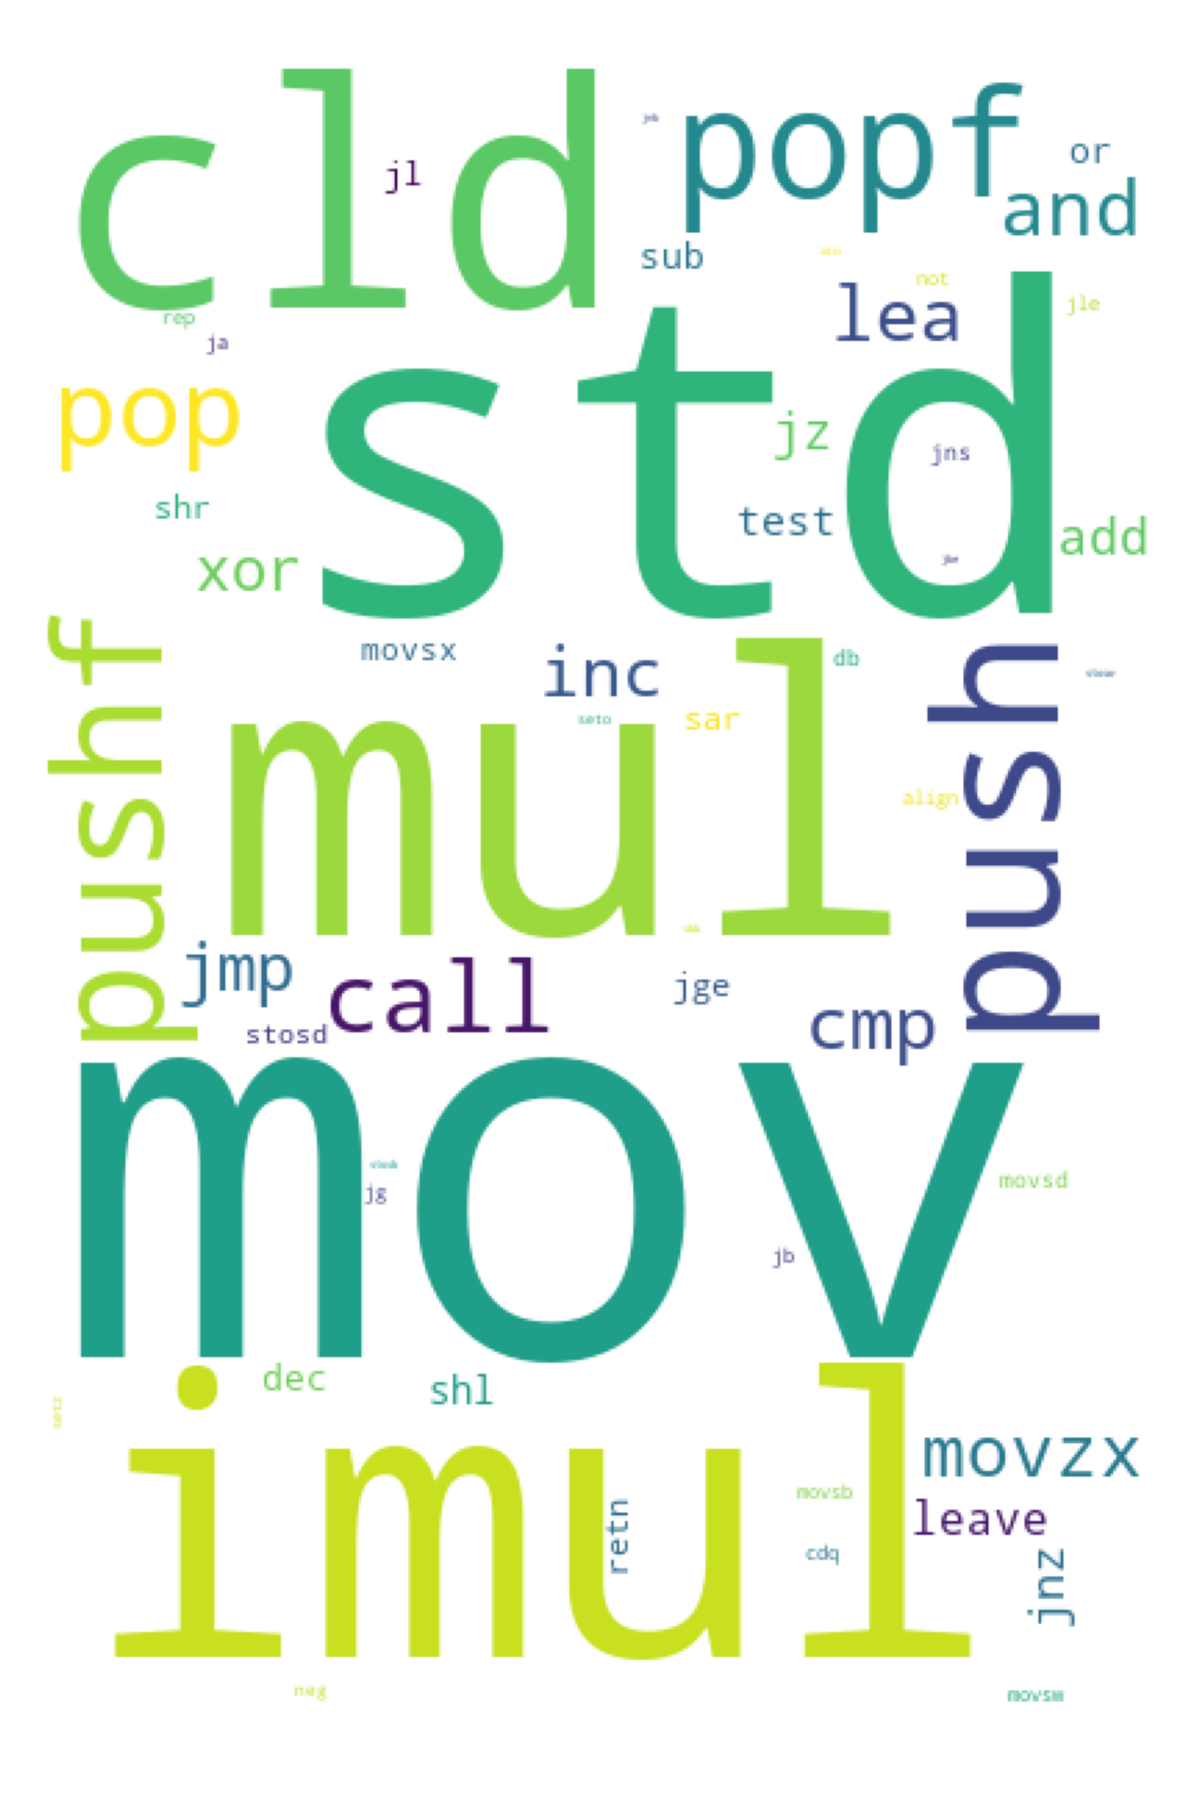
\includegraphics[width=0.95\textwidth]{%
			img/msoft_big/wordcloud/topic_06_wordcloud.png%
		}
		\caption{Topic 6.}%
		\label{fig:wordcloud_topic_6}
	\end{subfigure}
	\hfill
	\begin{subfigure}[c]{0.18\textwidth}
		\centering
		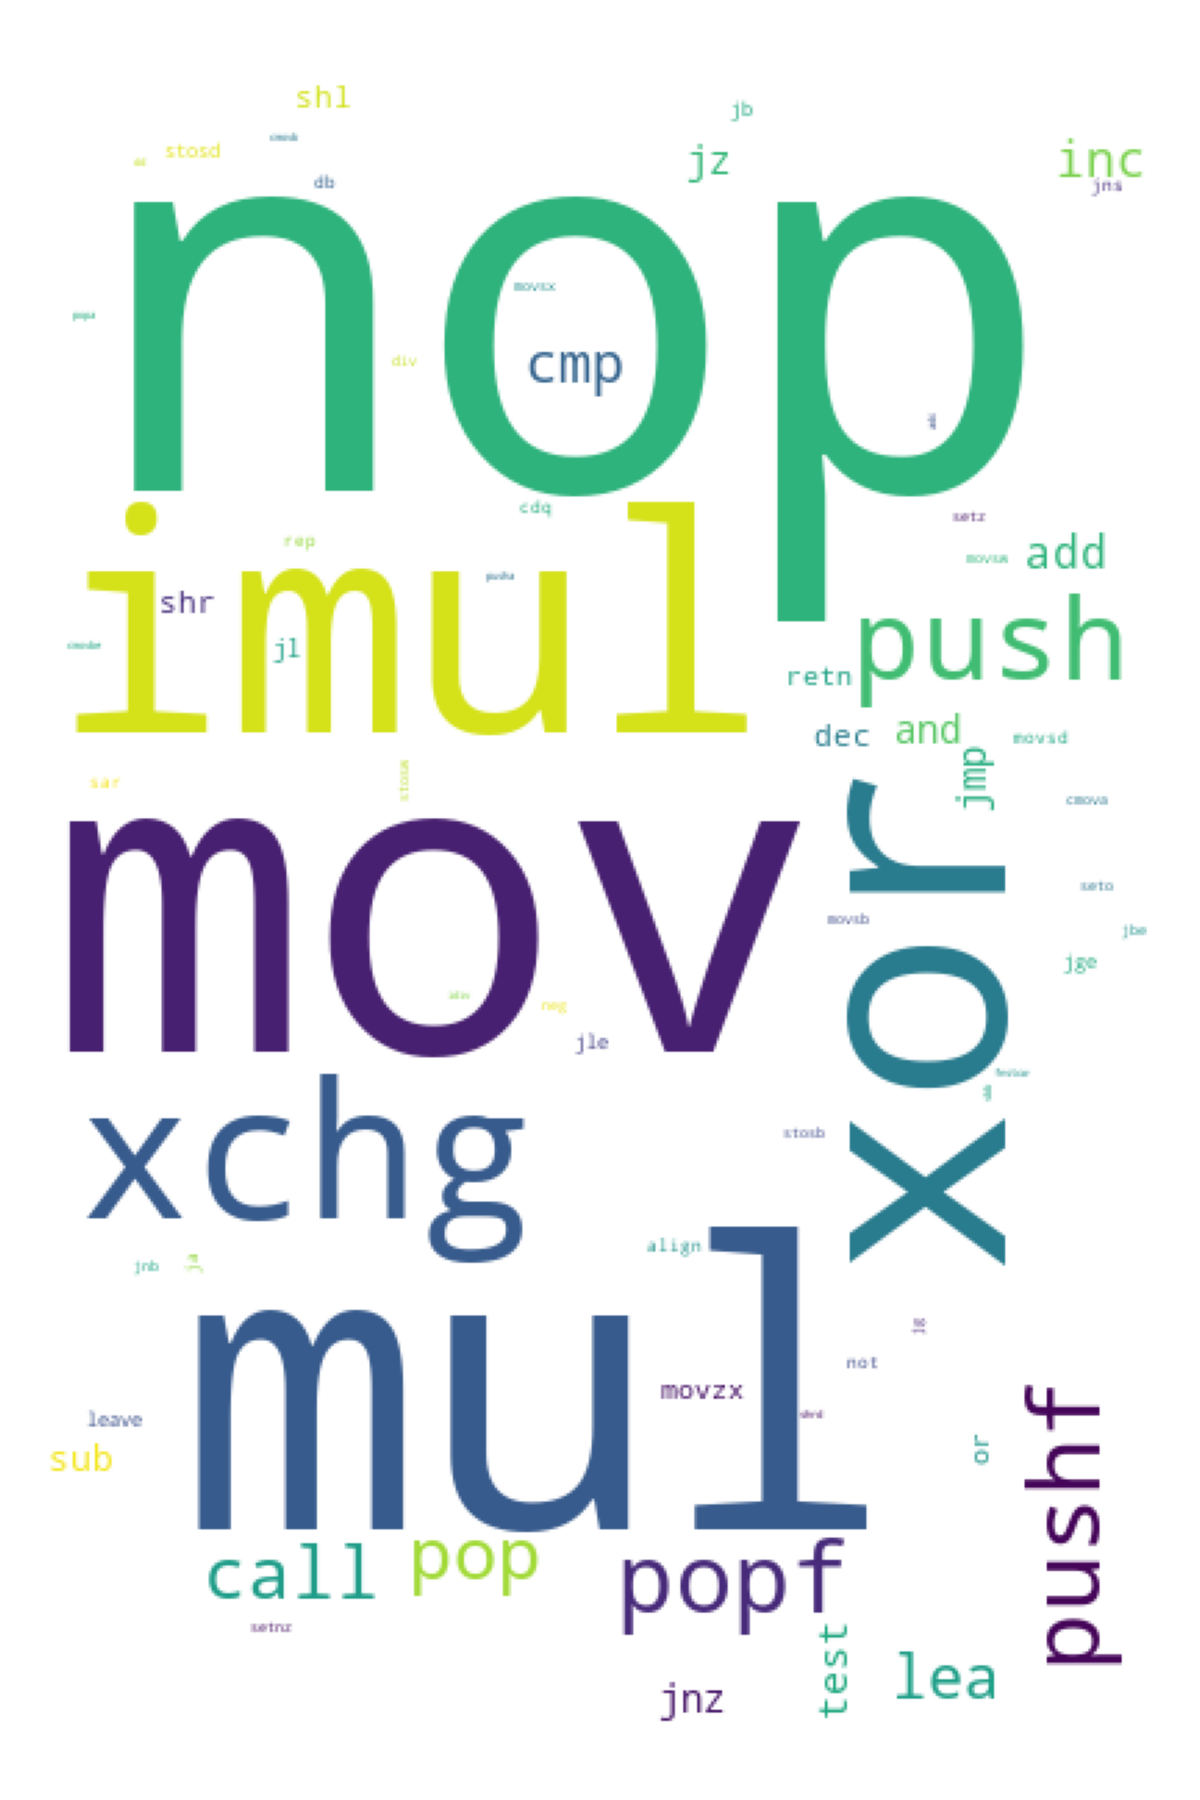
\includegraphics[width=0.95\textwidth]{%
			img/msoft_big/wordcloud/topic_07_wordcloud.png%
		}
		\caption{Topic 7.}%
		\label{fig:wordcloud_topic_7}
	\end{subfigure}
	\hfill
	\begin{subfigure}[c]{0.18\textwidth}
		\centering
		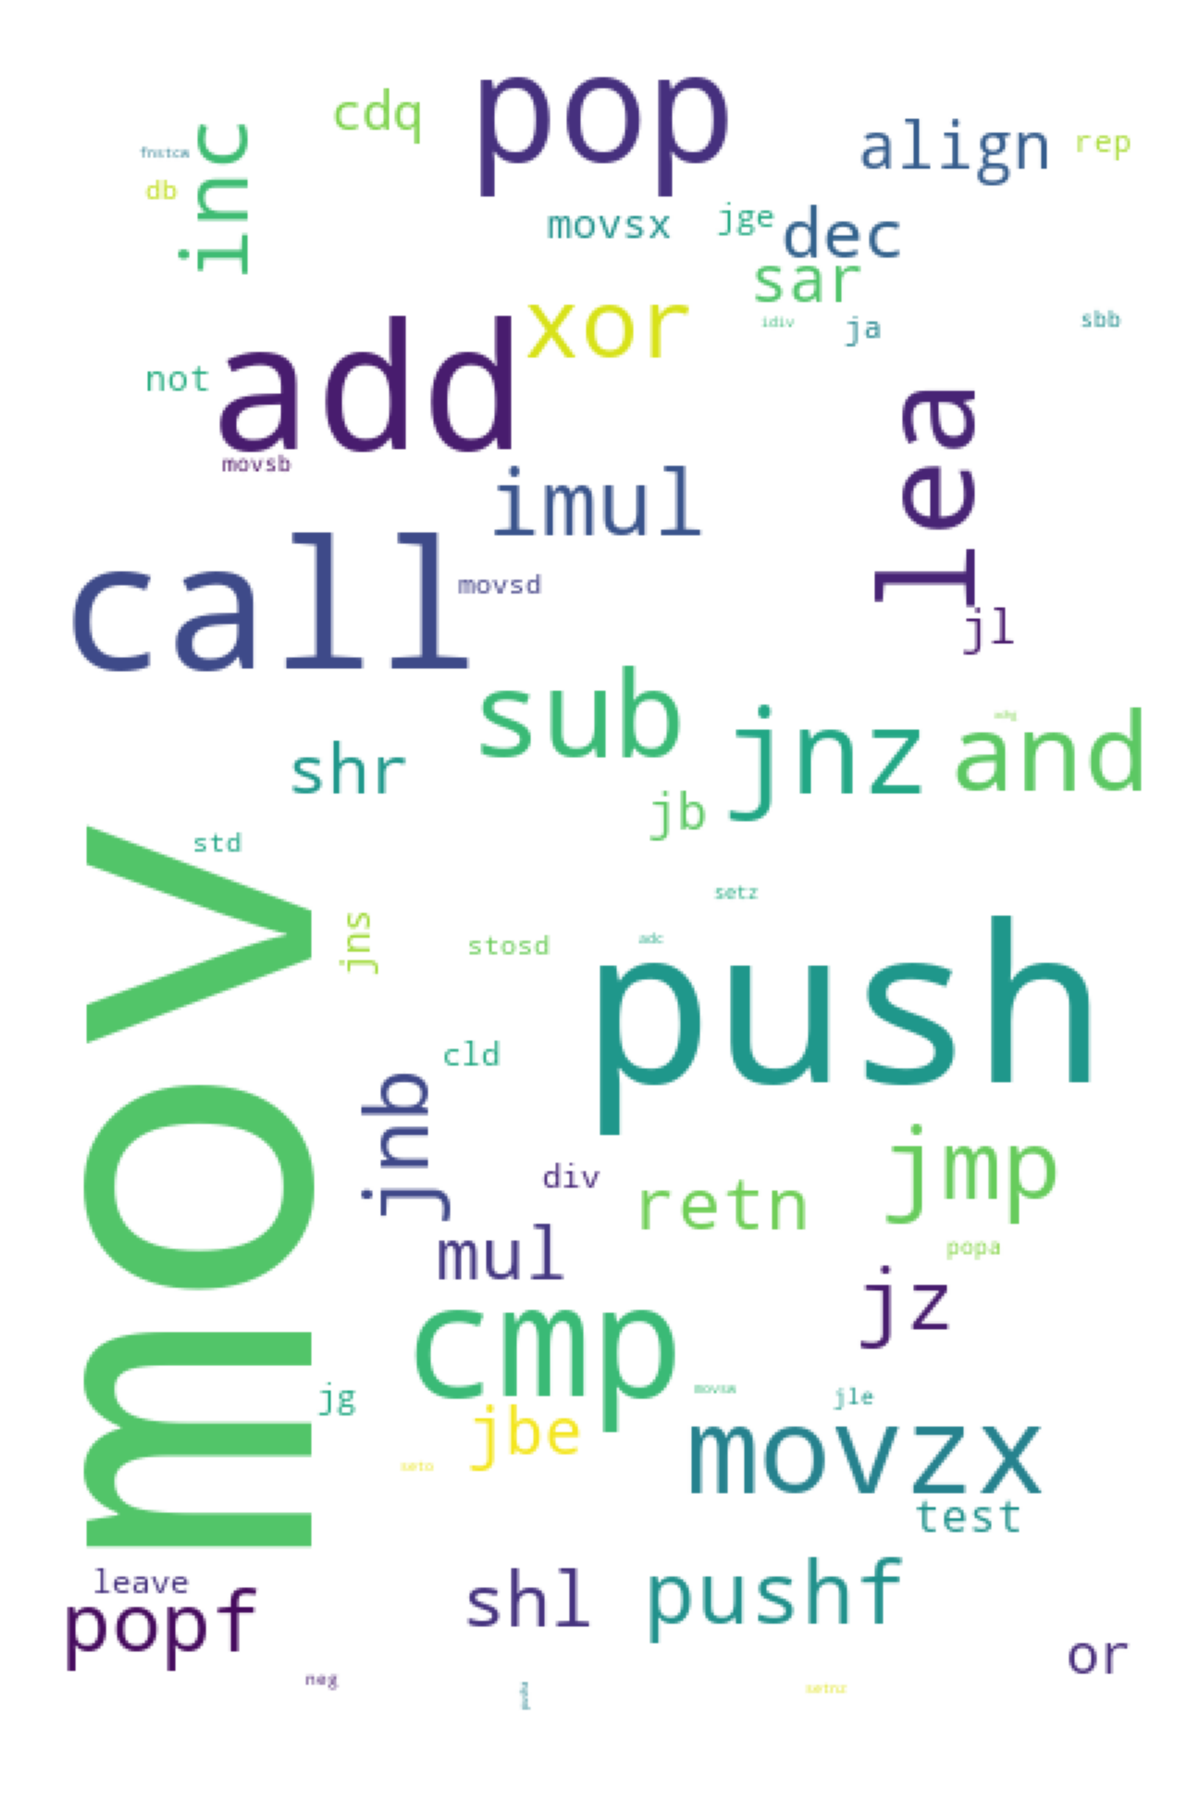
\includegraphics[width=0.95\textwidth]{%
			img/msoft_big/wordcloud/topic_08_wordcloud.png%
		}
		\caption{Topic 8.}%
		\label{fig:wordcloud_topic_8}
	\end{subfigure}
	\hfill
	\begin{subfigure}[c]{0.18\textwidth}
		\centering
		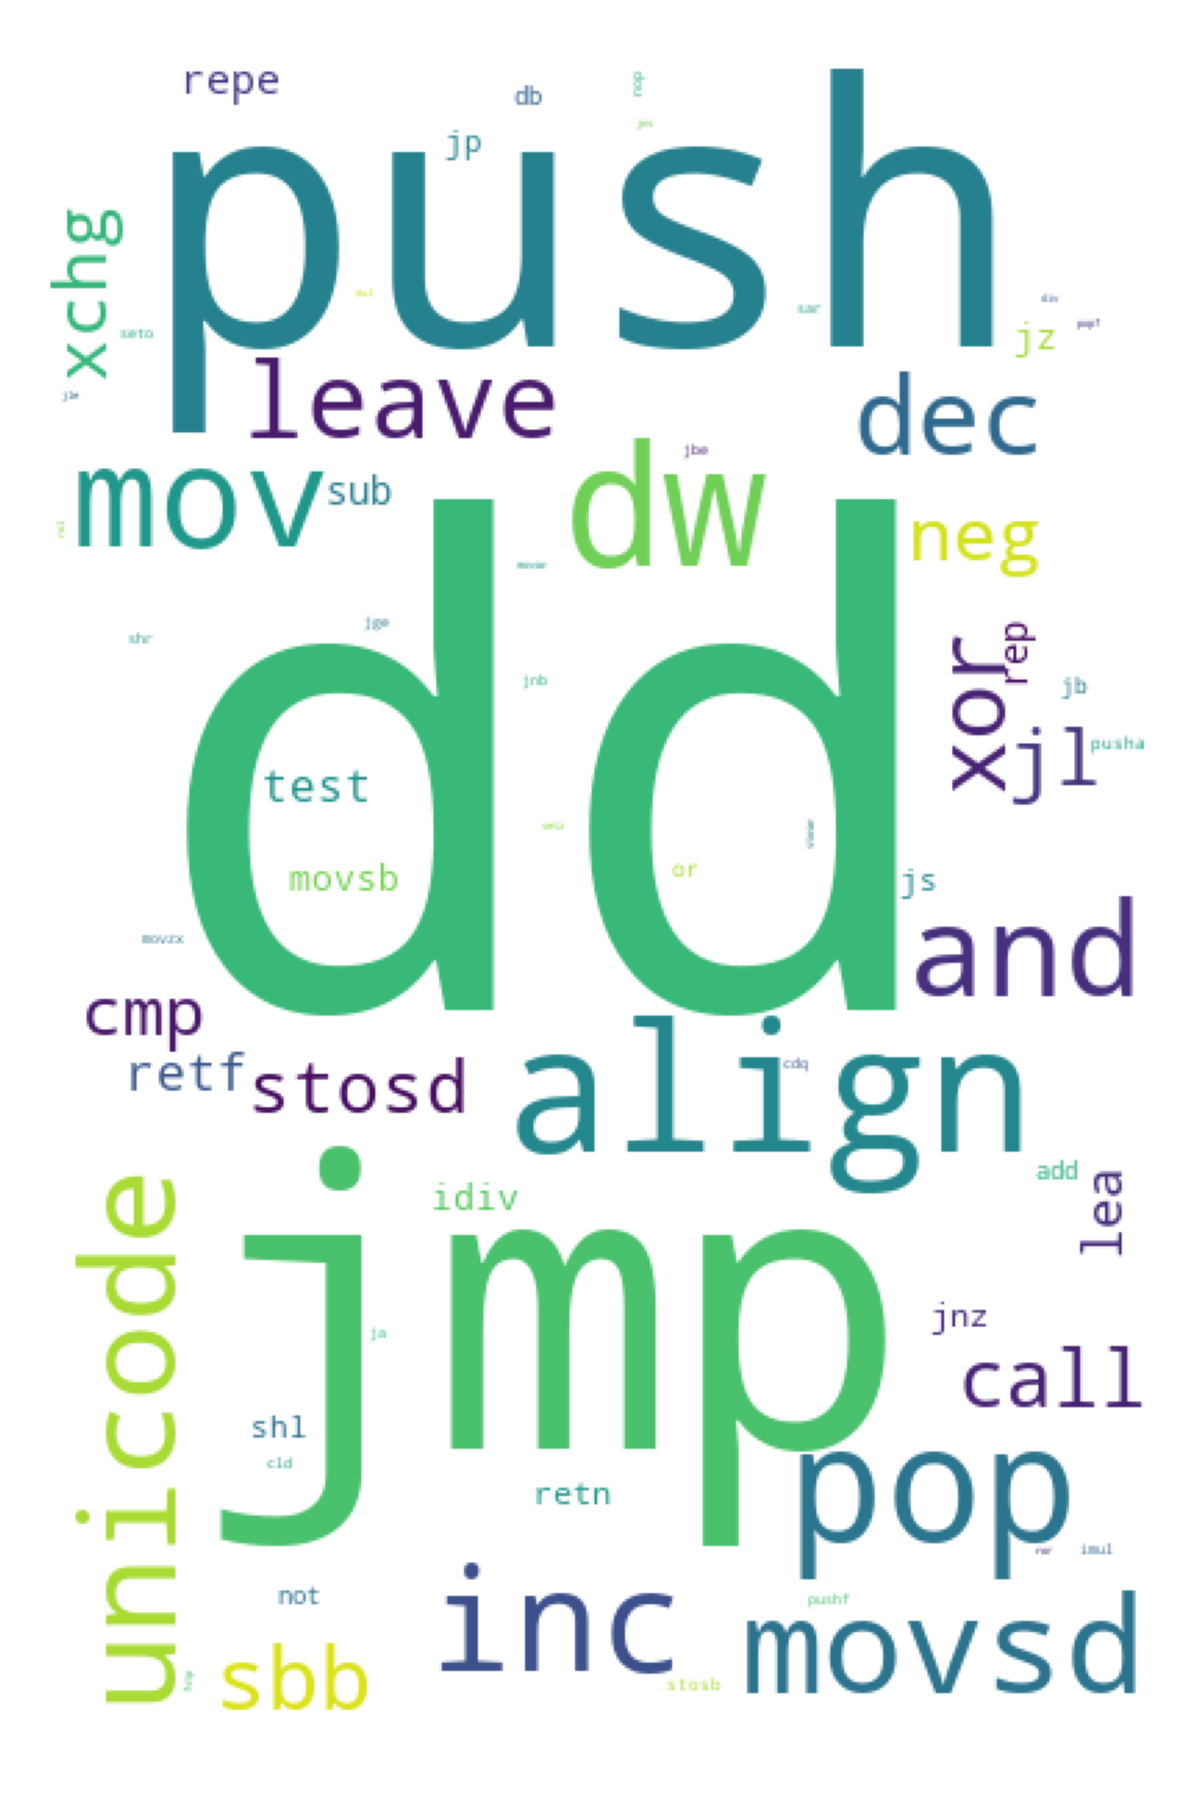
\includegraphics[width=0.95\textwidth]{%
			img/msoft_big/wordcloud/topic_09_wordcloud.png%
		}
		\caption{Topic 9.}%
		\label{fig:wordcloud_topic_9}
	\end{subfigure}
	\caption[Word cloud representations of LDA topics]{%
		Word cloud representations of each topic for a 10 topic LDA model fit on
		the Microsoft BIG 2015 dataset.
		The size of each opcode indicates its weighting in the topic.
	}%
	\label{fig:wordcloud}
\end{figure}

\section{Context Bit Model}%
\label{sec:mthd_context_bit}

\par In developing our first context-aware model, we started with a high-level
idea of how the data and features should be used.
Our original idea was to take several different sets of features from different
data collection strategies and combine them with contextual information in an
ensemble classifier.
First, the static disassembly of a file would be collected and filtered to a
sequence of static opcodes and fed through an LDA model.
Next, a dynamic assembly trace would be collected from each file and similarly
filtered to a sequence of dynamic opcodes and fed through an LDA model.
The final feature is a set of high level behavioral features.
The contextual information in this model is based on the physical context
of the system, which is derived from environmental information from sensor
data.
This data would then be interpreted by an environmental context model and fed
into the ensemble classifier.
A diagram of this context-aware model is shown in
\figref{fig:ensemble_context_bit}.

\begin{figure}[htb]
	\centering
	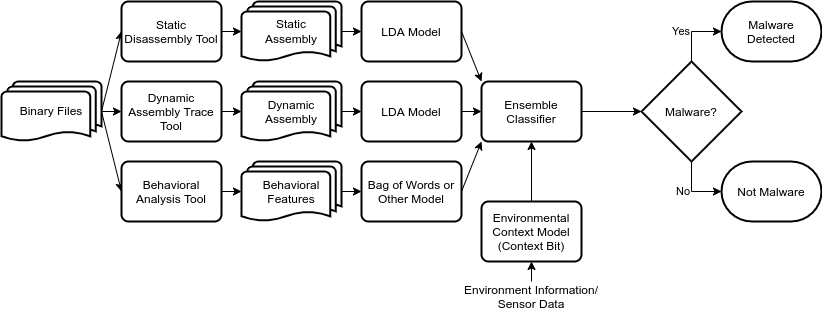
\includegraphics[width=0.95\textwidth]{%
		img/system_diagram_ensemble_context_bit.png%
	}
	\caption[Ensemble context bit model]{%
		Ensemble context-aware model with context represented as a context bit.
	}%
	\label{fig:ensemble_context_bit}
\end{figure}

\par While the ensemble system could provide more diverse features for
classification, there were limitations.
The biggest limitation was the speed at which the dynamic features could be
collected.
Because the dynamic features were not necessary to explore context in this
model, the ensemble classifier was removed, as with the behavioral analysis and
the dynamic assembly trace.
The simplified context-aware model is shown in \figref{fig:simple_context_bit}.

\begin{figure}[htb]
	\centering
	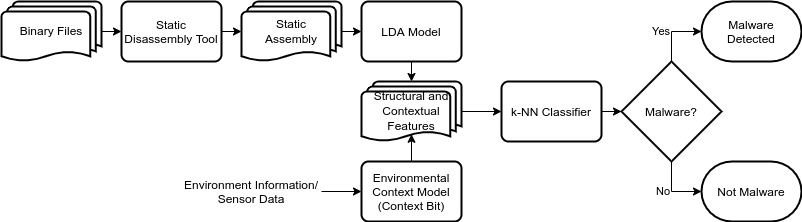
\includegraphics[width=0.95\textwidth]{%
		img/system_diagram_simple_context_bit.png%
	}
	\caption[Simplified context bit model]{%
		Simplified context-aware model with context represented as a context bit.
	}%
	\label{fig:simple_context_bit}
\end{figure}

\par Generating the sensor data and developing an environmental contextual
model would be difficult to generalize for our proof-of-concept model.
For this reason, we black-boxed the sensor data and context model and
simplified it to be a single bit to represent ``good context'' (0) and ``bad
context'' (1).
A context bit was randomly generated for each data point with a 50\% chance of
being either a 1 or a 0.
The context bit was then appended to the LDA features to form the feature
vector.
For example, if the LDA model has 15 topics, the feature vector would be
16-dimensional; the first 15 elements are be the 15 topic weights, and the
final element is the context bit.

\par The data was relabeled after applying the context bit.
For this process, we must take a different perspective on what the labels mean.
In the context-free model, each file was assigned either malicious or benign
with no contextual information.
However, when we consider the context of the system, whether or not a file is
malicious is dependent on the context the file is running in.
Instead, the files should be thought of as whether or not they are operating in
their expected context.
If a benign file is operating in a good context (context bit is 0), that should
be labeled as operating within proper context.
Likewise, if a malicious file is operating in a bad context (context bit is 1),
it should also be labeled as operating within proper context.
A file is labeled as violating its expected context if the nature of the file
does not match the context, meaning a benign file in a bad context or a
malicious file in a good context.
Files operating within proper context were labeled 0, and files operating
outside of proper context were labeled 1.
These new features were then classified using a k-NN classifier.
Because this model relies on only having two classes, we used the Das Malwerk
dataset described in \secref{subsec:mthd_das_malwerk}.

\section{Expected Behavior Model}%
\label{sec:mthd_expected_behavior}

\par While the context-aware model in \secref{sec:mthd_context_bit} addresses
physical context, we also wanted to attempt to address other areas of context.
For this model, we compared the expected behavior of a file with its actual
behavior.
Expected behavior of a program can be difficult to quantify.
For this case, we are considering the class label to indicate which type of
software we are expecting.
To ensure that all of the files within a specific class are actually similar in
functionality, we used the BIG 2015 dataset to test this model.

\par Like the model in \secref{sec:mthd_context_bit}, this model processes the
sequence of static opcodes through an LDA model to get the topic distributions.
The difference here is in how the context data is acquired.
Because the class label indicates the expected behavior of the program, if we
had a program which was mislabeled, that would represent a context violation
because the label does not match the actual software.
Referring back to the threat model, if the 3rd party software vendor gives us
a piece of software and says it's a video call program, we would expect it to
operate within similar context to other video call programs we have seen in the
past.
If the vendor gives us a program and says it is a video call program, but it
turns out to be a file sharing program, we should detect that the program is
not matching the behavior we would expect for a video call program and realize
that it is not operating within the expected context.

\par To simulate receiving a software which is not the type we are expecting,
we took the BIG 2015 dataset and changed half of the class types to an
incorrect type.
For programs which had the original type, we labeled those as operating within
proper context.
If the type was changed to an incorrect type, we labeled those programs as
violating their expected context.

\par The feature vectors for this dataset were formed similarly to the features
of the context bit model.
Instead of adding the LDA features and the context bit together, we added the
LDA features and the class type (with half of them changed to the wrong type).
Because the magnitude of the class type is arbitrary, we represented the class
identifier as a one-hot encoded vector.
The one-hot encoded vector ensures that all class identifiers are represented
with the same magnitude.
If the LDA model has 15 topics, the feature vectors would be 24-dimensional;
the first 15 elements are the LDA topic weights, and the last 9 elements are
from the one-hot encoded vector for the class identifier.

\newpage

\end{document}
